% SETUP
\documentclass[11pt]{article}
\linespread{1.25}
\usepackage[utf8]{inputenc}
\usepackage{graphicx, amsmath, array, graphics, amssymb, epsfig, psfrag, geometry, alltt, subfiles, blindtext, enumitem,float,pdfpages,multicol}
\usepackage[export]{adjustbox}
\usepackage{fancyhdr}
\usepackage{array}
\usepackage{hyperref}
%%%%%%%%%%%%%%  code listing
\usepackage{listings}
\usepackage{color} %red, green, blue, yellow, cyan, magenta, black, white
\definecolor{mygreen}{RGB}{2,94,33} % color values Red, Green, Blue
\definecolor{mylilas}{RGB}{170,55,241}

% MATLAB code insert
\lstset{language=Matlab,%
    %basicstyle=\color{red},
    breaklines=true,%
    morekeywords={matlab2tikz},
    keywordstyle=\color{blue},%
    morekeywords=[2]{1}, keywordstyle=[2]{\color{black}},
    identifierstyle=\color{black},%
    stringstyle=\color{mylilas},
    commentstyle=\color{mygreen},%
    showstringspaces=false,%without this there will be a symbol in the places where there is a space
    numbers=left,%
    numberstyle={\tiny \color{black}},% size of the numbers
    numbersep=9pt, % this defines how far the numbers are from the text
    emph=[1]{for,end,break},emphstyle=[1]\color{black}, %some words to emphasise
    %emph=[2]{word1,word2}, emphstyle=[2]{style},    
}
%%%%%%%%%%%%%%%%


\geometry{a4paper, top = 20mm, bottom = 20mm, left = 15mm, right = 15mm}

% Do we need a cover page?

% Headers
\pagestyle{fancy}
\fancyhf{}
\chead{ELEN90066 Embedded System Design - Final Report}
\cfoot{\thepage}

\begin{document}
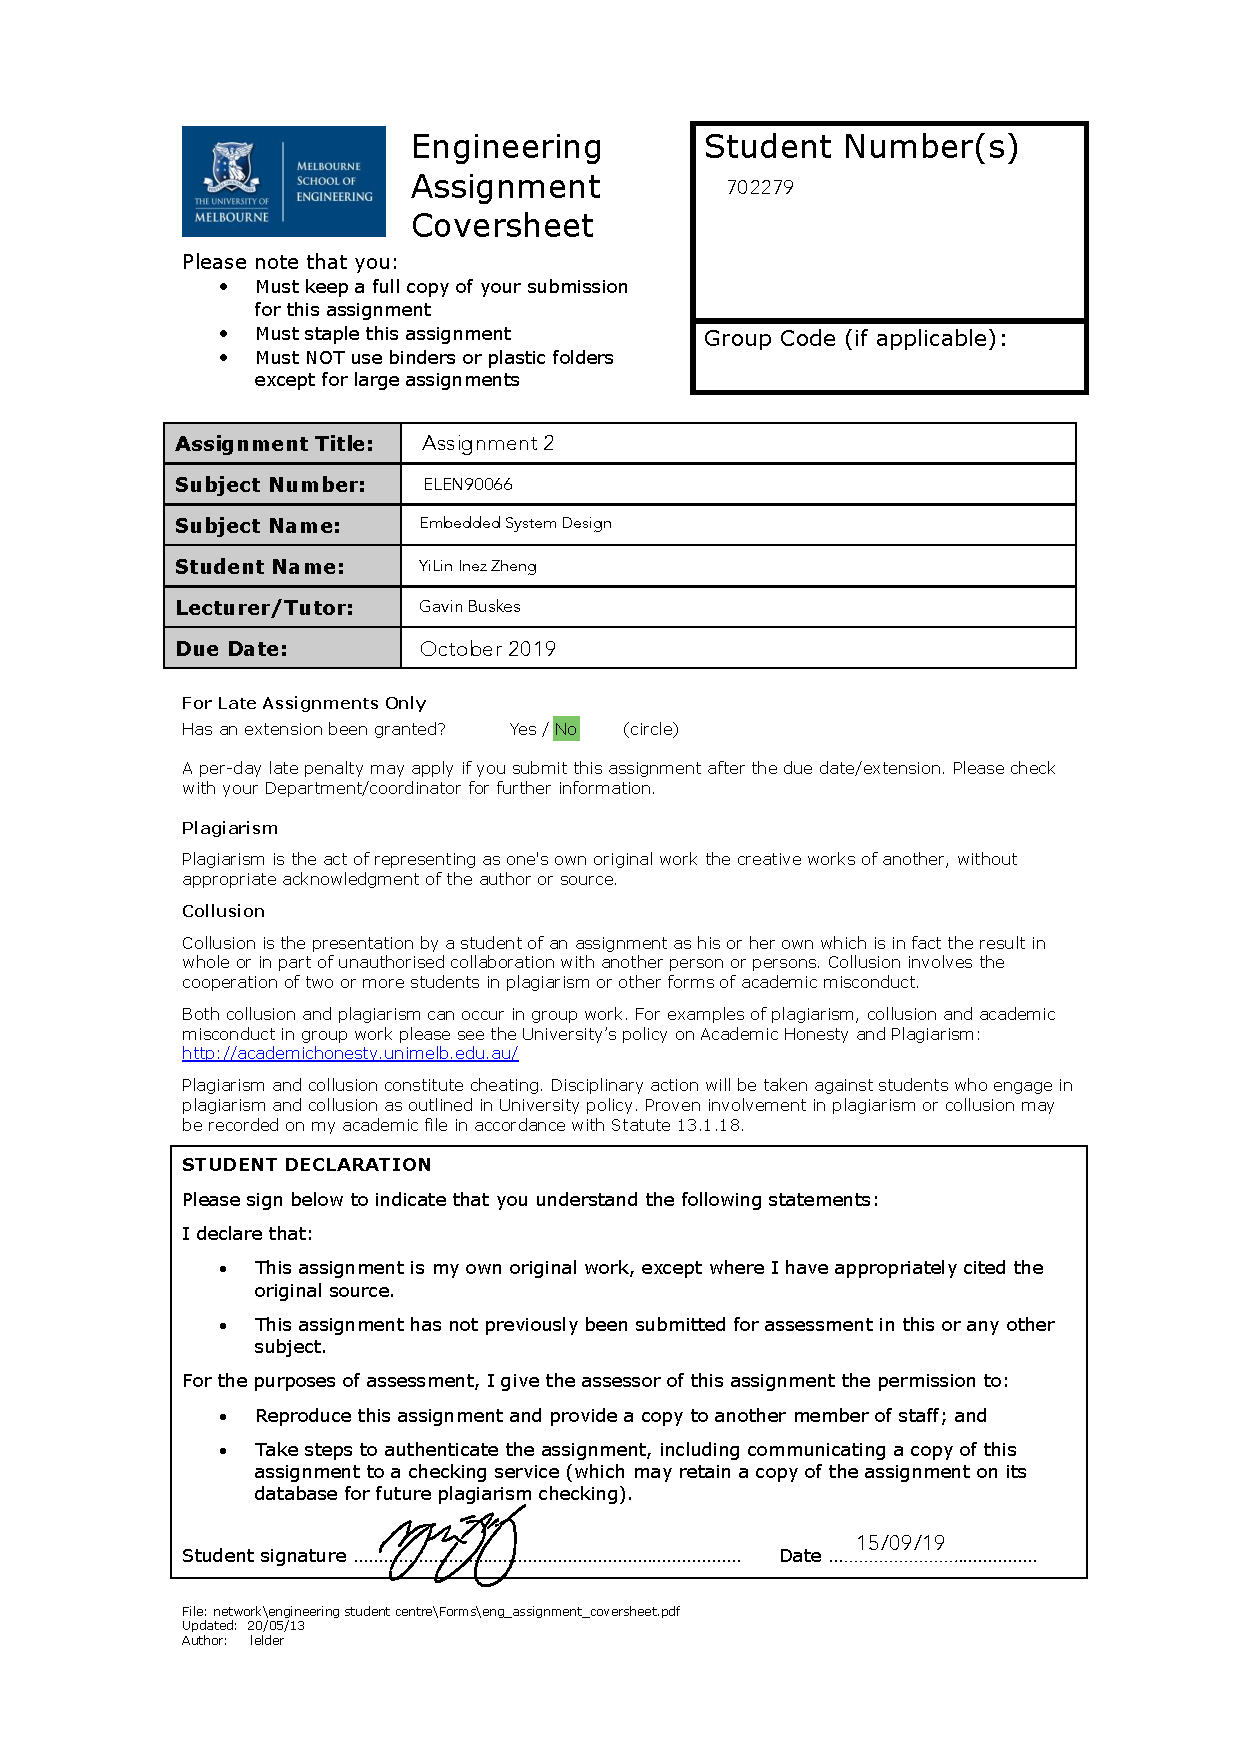
\includepdf{EngCSAss1.pdf}
% Title
\begin{center}
\textbf{\Large{Kobuki Obstacle Course Project - Final Report}}\\
Group 9: Craig Reid [756879], Xiuwen Peng [825801], YiLin Inez Zheng [702279], \\
Workshop: Monday 15:15pm - 18:15pm (Bigi), Due: 04/11/19  
\end{center}

%%% 20 page limit! %%%

\section{Introduction}
The Kobuki is an educational "turtle-bot" designed with hardware robustness and long lasting battery life to supply power to external devices. This allows us to connect the Kobuki up to a \texttt{NI myRIO-1900} reconfigurable I/O device and use the FPGA for implementing designs of a finite state machine (FSM) that navigates the Kobui through a 3x5m obstacle course. The arrangement of the myRIO on the Kobuki is shown in the Figure \ref{fig:kobuki}. The legend to the bottom right corner of Figure \ref{fig:kobuki} shows the orientation of the accelerometer ADXL330 used in myRIO. The forward direction for the Kobuki is the positive $x$ axis. 
\begin{figure}[H]
    \centering
    \includegraphics[width=9cm]{Kobuki.png}
    \caption{30cm diameter Kobuki with connected myRIO in bird's eye view}
    \label{fig:kobuki}
\end{figure}

\subsection{Project Requirements}
To successfully complete the obstacle course, we must follow the following requirements and rules:
\begin{itemize}
    \item \textbf{Play/Pause}:\\
    The Kobuki's action will be determined by it's 'B0' button. The robot shall only start when B0 is pressed. When pressed again all movement should be paused and the robot will resume upon another press of B0. The B0 button can also be referred to as the 'Play' button.
    \item \textbf{Driving}:\\
    The robot should stay level on the ground whilst moving at all times. The original positive $x$ axis position of the Kobuki at the start of the obstacle course determines the 'Ground Orientation', which the Kobuki should always follow. The ground orientation can only change after a power cycle, reprogram or restart of the robot or its embedded controller.\\
    \textbf{Challenges to overcome whilst driving}:
    \begin{itemize}
        \item \textbf{Obstacle Avoidance}\\
        The Kobuki should always avoid obstacles in the form of cliffs, wheel hazards, and objects whilst driving even during simultaneous or shortly successive encounters. After encountering obstacles, the Kobuki must be able to reorient and resume driving in ground orientation. The Kobuki is allowed to touch objects as long as it changes course immediately to avoid the obstacle. 
        \item \textbf{Hill Climb}\\
        The Kobuki must be able to climb up a hill, drive through the plateau and descend to a final stop on flat ground within 40cm of the bottom of the hill. The robot must be able to orient itself on the hill to execute an orthogonal climb or descent. At any time the robot must not go over the edge of the hill.
    \end{itemize}
    \item \textbf{Performance Specfications}
    \begin{itemize}
        \item \textbf{Rotation}: The Kobuki should not rotate more than 180 degrees.
        \item \textbf{Chattering}: Chattering and erratic movement should not be exhibited.
        \item \textbf{Abnormal Termination}: With the exception of power or mechanical failure, the robot should not stop at any time.
        \item \textbf{Obstacle Hugging}: The Kobuki is not allowed to repeated encounter the same obstacle for navigation.
        \item \textbf{Timeliness}: The obstacle course should be completed within 60 seconds.
    \end{itemize}
\end{itemize}

%%%% Design
\section{Analysis and Design}
Navigating the obstacle course using a Final State Machine introduces flexibility in control and a level of autonomous decision making by the robot in correspondence to sensors and actuators.

\subsection{Kobuki Sensors}
%A basic description of the sensor data available to myRIO and how it was used in your algorithm
With a variety of sensors available on the Kobuki, we chose to use applicable sensors for our obstacle navigation. Table \ref{table:kobuki_sensors} shows the sensors we used in our design and the obstacle course specifications that the sensors will help achieve.
\begin{table}[H]
\begin{center}
\begin{tabular}{ |l|c|c|c| } 
    \hline
    \textbf{Sensor} & \textbf{Number} & \textbf{Target Specification} & \textbf{Notes} \\ 
    \hline
    Wheel Drop Sensor & 2 (left, right) & Maintain ground contact & \\
    \hline
    Cliff Sensor & 3 (left, center, right) & Hill climb edge avoidance & \\
    \hline
    Bumper & 3 (left, center, right) & Object avoidance & \\
    \hline
\end{tabular}
\caption{Empirically determined parameters for the Quanser Aero system} \label{table:kobuki_sensors}
\end{center}
\end{table}

\subsection{Accelerometer ADXL330}
To detect inclination and reorient the Kobuki whilst on the inclined hill, we used the accelerometer on the myRIO instead of the gyroscope that came with the Kobuki because the accelerometer offered readings in 3 axis ($x$, $y$, $z$) in comparison to the single axis reading from the gyroscope.\\

\noindent Using the accelerometer readings we calculate the pitch and yaw angle with respect to the Kobuki's $x$ and $z$ axis. 

% mapping etc. how it always results in 'g'
% enter stuff about pitch and yaw angle calcs. references?? biblatex
% thresholds and tuning
% accelerometer sensitivity + LPF

\subsection{Final State Machine}
%A complete FSM diagram (including pause states) of the robot algorithm using the notation covered in the lectures. If you use an Extended state machine, or state refinements, you must show all states, variables and transitions.
We aim to make the state machine simple and efficient leading us to consider hierarchical design to avoid redundant states as well as system variables to reduce and simplify states. 

\textcolor{blue}{Brain dump:\\
- Accelerometer angle readings, pitch and yaw\\
- LPF for accelerometer refer to incline plane doc, accuracy of angle calculations etc.\\
- efficiency of code: hierarchical state machines, spaghetti code vs. function pointers\\
- threshold checking for hill climb, simulation vs reality
}


%%%% Sims and testing
\section{Implementation and Testing}

% Simulation results, and how the simulation was shit.
\subsection{LabView vs. C/C++ (Eclipse)}

\subsection{Obstacle Avoidance}

\subsection{Hill Climb}
%% harder to test for, accel readings etc. 
% - curved movement 
% - kp feedback controller

\section{Validation}
% some end thing about our performance after it hits challenge requirements
% - final workshop result

\section{Discussion}
% refer lectures!
% talk about improvements

\textcolor{red}{The report must contain (but is not limited to):\\
• a complete FSM diagram (including pause states) of the robot algorithm using the nota- tion covered in the lectures. If you use an Extended state machine, or state refinements, you must show all states, variables and transitions\\
• a basic description of the sensor data available to the myRIO and how it was used in your algorithm\\
• your design procedure (this could include work from earlier workshops)\\
• your testing procedure (this could include simulation data or screenshots)\\
• your validation procedure (this could include reliability or reachability analyses)\\
• the outcome of the run in the final workshop\\
• a discussion section (how you applied knowledge from the lectures, what you would im- prove in the future)
The report is to be no more than 20 pages in length. A marking rubric for the report will be available on LMS.
}

\end{document}